\documentclass[11pt,a4paper]{article}
\usepackage[utf8]{inputenc}
\usepackage{graphicx,enumitem}

\title{Ray Tracer application Final Report}
\author{A. Manolache, N. Shirvanian, A. Georgiou, S. Orazgulyyev, S. Moraby}
\date{February 5, 2018}
\begin{document}
\maketitle

\section{Introduction}

This report will achieve to provide a detailed and extensive description of our ray tracer design and implementation for the Group Project module. It will also have an outline of the goal achieved and the difficulties that we faced as a group throughout the project. Moreover, an analysis of our team's organization will be provided. Finally, the evaluation for our project's architectural design will be carried out so that the motivation is well understood followed by the peer review. 

\subsection{Project Specification}

The goal for this project is the design and implementation of a well-functioning ray tracer. Provided the above, our assigned team has come together to take on the challenge and produce a final software with at least the minimum necessary specifications. 
These specifications include a back end and a front end (GUI), that need to operate with the following requirements according to the project’s description: 

Back end:
\begin{itemize}[nosep, wide=20pt, leftmargin=*, after=\strut]
    \item Receive an input of a scene 
    \item Render than input as a PNG
    \item Allow the user to specify the size of the PNG
    \item Allow the user to specify the name of the PNG file
    \item Support operation with 3-dimensional coordinates (x, y, y)
    \item Consequently allow for rendering of multiple basic shapes
    \item Allow rendering with multiple light sources 
    \item Allow rendering of different textures 
    \item Operate in a reasonable amount of 
\end{itemize}

GUI:
\begin{itemize}[nosep, wide=20pt, leftmargin=*, after=\strut]
    \item Support the sketching of the scene that will be saved to a file and input to the backend
    \item Provide all shapes, colours and setting that the backend supports
    \item Operate in reasonable amount of time 
\end{itemize}

Consequently, we arranged a reasonable Gantt chart that aided us in the completion of each stage in the project, in a timely manner. The Gantt chart as seen in Figure 1, was carefully constructed in way, that would allow for plenty of remainder time to be used in the “worst case scenario”, where more time would be needed to be allocated for certain tasks. Following these guidelines the team managed to accomplish the completion of the software and its supporting report that provides additional information regarding our process. 

\begin{figure}[h]
\centering
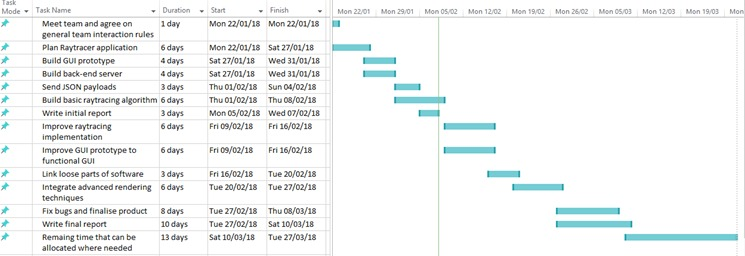
\includegraphics[scale = 0.4]{ganttchart.jpeg}
\caption{Grantt Chart}
\end{figure}

\subsection{Achievements and the Work}

Throughout these past six and a half weeks, starting from the day after our initial presentation, our team has managed a number of achievements that shall be briefly discussed in this section and more thoroughly in the following ones.

Firstly our group was divided in two parts, the front end (GUI) development and a back end (ray tracer algorithm) development. Both parts took up equally several days and similar effort to complete in time and to our standards. The front end developed by Nima, went from a prototype of a GUI to a functional and beautifully designed user-friendly interface that allows the sketching of a scene with multiple shapes, colours and additional lights and texture options. With Suleyman’s help, the GUI was finally connected to the back end, sending the user’s input from the GUI to the back end for the ray tracing operation. In turn, the back end takes in the input from the GUI, such as the shapes, colour, lights and texture and performs the ray tracing of those shapes. Consequently a rendered image is returned and can be saved as a PNG file with a name that is specified by the user. 

According to the Gantt chart ( see Figure 1), the completed software should have optimally been ready thirteen days before the deadline. This would allow for the allocation of the remainder time, to parts that required fixes or updates. Thankfully, the remainder thirteen days before the deadline where crucial because we indeed required more time to complete certain tasks, just as we predicted in our “worst case scenario” thinking. Following that, a collection of JUnit tests was conducted in order to verify that our code actually executes the expected behaviour and results in the expected state. Two advanced rendering techniques namely anti-aliasing and super-sampling were also integrated to our ray tracing application while bugs encountered during testing phase were dealt with the appropriate changes.

At last, the rest of the report will provide an explicit explanation of the requirements and design section. The implementation of our ray tracer application is also discussed in details as inspired by the relevant research work carried out. The conclusion of the report will be based on a discussion on the evaluation of the performance and functionality of the application.

\section{Review}
A thorough research was done before starting to set the requirements for our ray tracer application as well as for the design and implementation phase. In this section, all relevant work will be displayed along with a brief explanation of how it helped.

\subsection{Initial Research}
Tutorials were used as reference to get an intuition on the simulation of the ray tracer and on how to render shapes by reproducing pixels in an image plane through a trajectory of light. Before deciding on a specific design for our ray tracer, we had to thoroughly research the subject. From our initial research we came across the following video tutorials that really helped us understand the concept of the project and what was expected from us to do. Consequently, we started applying these tutorials to better understand the implementation of the method they were explaining. 
The very first tutorial we watched was a series called “Rendering 101” which provided thorough explanations on the basics of a ray tracer works and how light reacts with the objects that the ray hits  (Khan Academy, 2018). The series also included a number of tasks that the user can experiment with by manipulating certain parameters (specular, diffuse, angles etc.) which added to our understanding of what each of those parameters do.
 A particularly helpful source that we researched, was a book called “ Ray tracing from the ground up”, that contains a lot of information on how we could implement a ray tracer from scratch; we turned to that book a number of times after a number of dead ends (Suffern, 2007). 
Even though we decided that the coding of the back end should be done using Java programming language, we came across another very helpful tutorial series, “”RAYTRACER FROM SCRATCH IN C++” that uses C++ programming language for its implementation (YouTube, 2018). Those tutorial series were particularly useful as well, along with all the other sources of information, implementation and inspiration that we took into account when we started the implementations of our ray tracer application.

\subsection{External Libraries}

\begin{itemize}[nosep, wide=20pt, leftmargin=*, after=\strut]
    \item Jackson API (library to serialize or map java objects to JSON)
 Even though Spring already provides the deserialisation of JSON  it only provides it for primitive types (e.g. int, string etc.), but our POJO contains custom objects such as Figure and Light. Therefore, we needed to use Jackson to deserialise embedded custom objects.
 
    \item JUnit5 was used for testing along with Mockito to facilitate the mocking process
    \item JQuery was used to facilitate the manipulation and selection of DOM objects 
    \item Bootstrap was used to enhance the styling of the GUI 
    \item Springboot was used as a foundation for the application which ensured communication and injection
    \item Three.js is a JavaScript library that was usd to graphics on the GUI 
\end{itemize}

\section{Requirements & Design}
The definition of our project, initially started from the minimum requirements specified, mentioned in the section 1.2 of this report. During the researching stage of our project, which was the very first week after our team allocation, we initially tried to understand how the requirements as shown in section 1.2, could be implemented. This researching period was very enlightening for us since we came across a number of different tutorials, that helped us in understanding the reasoning and also the mathematics and even physics behind a ray tracer algorithm (see section 2.1). During that initial period we also started experimenting using the help of the tutorials in section 2.1, to better grasp the thinking behind the implementations that we had seen in those tutorials. 

After our research we started discussing ideas on the design of the project, what languages we should use, how we should approach the problem and what additional requirements and features do we want our project to contain. We wanted to implement a number of different shapes that the user can add to their scene, different lights, colours and at least one more texture (surface material) that the user can select from. The requirements we decided on, in turn, complicated the project but we were all ready to take on the challenge and develop a project that we have never attempted before. Consequently the requirements we added for our project, complimented the design approach we had already decided on therefore the accommodation of the new features was, of course, not easy but applicable.

Furthermore, a very specific obstacle we faced while the software development, was the mathematics and physics behind the implementation of every shape, how the lighting, shadowing and reflection would react with those shapes and how the front end would manage to render it successfully. We managed to figure out most these issues through our exhaustive research, that contained a number of different implementations of ray tracer applications. We looked through all the GitHub repositories to get an idea of how we could implement the different shapes, lights, shadows, reflections and how the ray tracing operation could be applied to each shape.
Furthermore, the following parts of this section will aim to explain the approach we decided to take, why we decided on that approach and the requirements that we set for our project.

\subsection{Requirements}
After an exhaustive research we came to a final decision regarding the requirements that we wanted to set for our project. These requirements included additional features for the ray tracer application, hoping for a more fun and adequately complex implementation and result. Such additional requirements according to the standards that our team has set and wanted to achieve during this group work, are the following: 

Back end:
\begin{itemize}[nosep, wide=20pt, leftmargin=*, after=\strut]
    \item Operate in a reasonable amount of time - Use of multithreading 
    \item Allow rendering of circles, rectangles, cubes, spheres, toruses, cones, cylinders and triangles (total of 8 shapes)
    \item Allow rendering of two different textures (normal texture and checkered texture) 
    \item Use of Phong reflection model (Ambient Lighting + Diffuse Reflection + Specular Reflection) 
    
    \begin{itemize}[nosep, wide=20pt, leftmargin=*, after=\strut]
        \item Ambient Lighting - The light that already exists 
        \item Diffuse Reflection - Reflection that happens when the hit of the ray gets dispersed across many angles
        \item Specular Reflection - Regular reflection of light from the surface of an object
    \end{itemize}
    
    \item Use of shininess -  Polished feeling of the surface of an object 
    \item Use of Super sampling - A method of anti-aliasing (spatial) used to remove harsh edges from the rendered image. 
    \item Use of shadows for objects (when shadows should be present) 
\end{itemize}

GUI:
\begin{itemize}[nosep, wide=20pt, leftmargin=*, after=\strut]
    \item Allow camera positioning and control 
    \item Allow user to zoom in and out of the rendered image
    \item Allow user to specify their options for each shape 
    
    \begin{itemize}[nosep, wide=20pt, leftmargin=*, after=\strut]
        \item Choose how to name the shape they want to add
        \item Specify the shape’s dimensions
        \item Specify the shape’s color
        \item Specify the shape’s surface texture 
        \item Specify the shape’s shininess 
        \item Specify the shape’s dimensions ( different for each shape)
        \item Specify reflection 
    \end{itemize}
    
    \item Allow user to specify their options for the lighting 
    
    \begin{itemize}[nosep, wide=20pt, leftmargin=*, after=\strut]
        \item Specify light colour
        \item Specify light direction
        \item Allow the naming of the light object 
        \item Allow adding of multiple lights
    \end{itemize}
    
    \item Allow user to add and remove shapes from the canvas 
    \item 360 degree rotation of the object 
    \item 3D display of the object 
    \item Specify output size 

\end{itemize}

\subsection{Design}

The approach that the team decided on for the design was a MVC (Model - View - Controller) architecture. The reason we decided to go about the project from this architecture angle was, as mentioned in our initial report, to facilitate better flexibility through the ability to construct the separate components of our software but keep everything interconnected. Our decision to integrate Spring Boot into our project arrived from the need to quickly achieve an out of the box, configurable project that will use the Spring Framework including Spring MVC. The motive behind our decision to implement Spring Framework within our software was based on the framework’s capacity to build decoupled systems by wiring different components together using the dependency injection pattern. This worked coherently with our approach to develop our system using an MVC architecture and supported our initiative to segregate the service and web layers, consequently making the development life cycle of our system substantially easier. Spring also supplies hooks for Restful Services, which we used to send a JSON payload, triggered via an Ajax within the GUI, containing the information that we need, to render a scene full of geometric objects, by feeding it to our ray tracer algorithm. 

Our ray tracer algorithm was developed using Java 8 along with extra integration frameworks and a Tomcat server. Tomcat is an open-source server that is very lightweight in the sense that it loads rather fast but apart from that, the reason Tomcat is being used for this project is because it came integrated with the Spring framework. Furthermore, an Ajax call will trigger the sending of user input from the GUI to the back end in a JSON format. Then Jackson API is being used to de-serialize the JSON payload to a Plain Old Java Object (POJO). Consequently the values are then passed to a method which renders an image and outputs the result to a buffer which is then converted to a PNG image that is sent back to the user. Overall, the design that was established in the beginning did not have to change but we did have to use the Jackson API for the operation explained above. 

\section{Implementation}
This part will define our systematic approach to effectively build our software application from the front end to the back end, the communication between the front and back end and the testing. The main component behind the successful operation of our Ray Tracer web application was the implementation of the GUI, the Rest Full services and the ray tracing algorithms. 

Our system uses object-oriented programming to model objects, such as camera and geometric shapes, with the help of vectors and coordinates in a three-dimensional space. The ray tracer algorithm takes an image containing geometrical objects that can be added by the user from the GUI. For each pixel a ray of light is hit into the scene of the image to obtain an intersection between the light and the object. The direction of the ray is extracted by following the line of intersection from the position of the camera from the pixel of the object.

The aim is to establish whether any objects have been hit from our image scene and get its colour by using its surface normal and the light. For each shape, the distance of intersection is inferred by the general equation of that particular shape, along with the parametric definition of the ray in order to solve the resulting systems of equations using linear algebra. The colour is extrapolated by stretching the ray until the point of intersection and then a viewing vector can be extracted to obtain the normal of the point of intersection. Our algorithm then shoots rays towards each light source to establish its visibility. By default, the distance from the intersection is set to infinite and light will be classified as being visible if there is no intersection with an object within an epsilon away. As long as the light is visible, we measure the amount that hits the primitive at the intersection point by determining the angle to the light source from which we infer the colour. If our ray manages to intersect multiple objects, then the algorithm will select the shape with the minim distance from the camera. The tracing of the ray is done recursively so that after the ray manages to hit an object we continue tracing the reflected ray from that point.

GUI:

There is an initializer function that makes a scene object for the three.js library, the camera, the initial attributes, an extra scene and camera for the axis helper, defines the rendering loop, defines the behaviour associated with clicking on different buttons. 

There is a general shape object containing common values for all types of shapes (e.g position, reflection, etc). For the other shapes there exists a class inheriting from the general shape object. Each of these has a function to export its own properties as JSON compatible and converted with back end shape attributes. For some shapes it includes many geometrical components.

There is a local scene object which has a three.js scene inside, a list of shapes (local objects), list of lights and adding functions for each shape. Each adding function adds a shape in the local list and simultaneously in the three.js scene. It has a function to integrate all JSON attributes of objects and send them to the Back end via AJAX call.


\subsection{Testing}
A java-based library namely mockito was used for testing in conjunction with JUnit in order to create and configure mock java objects. Therefore allowing to productively test our system and increase the quality of the code. Our goal was to test for the actual outcome against the expected outcome using assert statements that compare the results.

Camera test and ray test 
Geteye, getlookat, getupdirection, getdirection, getviewplaneup

Shapes test 
Circle, Cone, Cube, Cylinder, Rectangle, Sphere, Torus, Triangle

Service test
Ray service, Ray tracer

\subsection{Performance issues & Solutions}
Regarding performance of our ray tracer application, we have implemented multithreading in the back end. We used it to amplify our performance by allocating multiple tasks to threads to be executed concurrently. This has been achieved by creating a ThreadPoolExecutor which provides a good amount of flexibility in defining thread pools due to its versatility. As a consequence it allows us to define executors and gets resources from the CPI.

Another way of maximising the performance is by using JSON to pass values from the front to the back end which is a lightweight and flexible method to transfer data. 


\section{Teamwork}
This section of the report, is dedicated in explaining and informing the reader of the different communication methods used within the group, as well as the team effort put towards the completion of the project before the deadline. All forms of communication between the group members, will be mentioned and briefly explained regarding the effect that they had in the development of the project. 

\subsection{ Working together}
The overall team work during the development of the software, has been rather smooth and enjoyable, even under stressful and difficult circumstances. We consider that the prosperous nature of our group’s working together, could be credited to the very fortunate random assemble of our team. Our team dynamic and chemistry with each other was pivotal for the successful development of the project and the communication between the team members. Along with our complimentary chemistry as a group, we also came together using a number of different communication mediums and face-to-face meetings every single week. Our regular meetings assured the timely progress of both the design and the implementation of the ray tracer and its GUI as well as the quick detection of bugs and their recovery with fixes. 
Additionally, each member had a purpose, a task to fulfill, that contributed to the completion of the overall goal; the assigned project. However, in addition to the individual tasks that each team member had been assigned, all five members were available at any time needed, to jump in and help with different ideas on the implementation or any errors that needed fixing in the code. 
Furthermore, we were overly lucky to not have caught ourselves in any sort of uncomfortable arguments or severe conflicts. That is, in terms of our communication as a group and the way we expressed our ideas when it came to deciding on an approach for the implementation. We came across healthy disagreements as expected from any team, but our team members were always respectful of each other. No heated arguments occurred and we always remembered to follow the “healthy communication” guidelines, as mentioned in the section 3.2 of our initial report. 
Finally, the following parts of section 5 of this report, will be explaining the different tools we used for our team communication and the development of the project. 


\subsection{GitHub}
Out of all tools that we used for our group work, we can admit that GitHub had been the most challenging of all. During the first four weeks of our group working, it is a fact that we were worried using GitHub due to the fact that we had no essential previous experience with the specific platform. We came across a number of issues, while trying to utilize the platform, that led to concerns regarding GitHub, which in turn made it easier for us to not use GitHub as often and instead only use it when we had something substantial to push. However, after a few weeks of practise we managed to overcome our fear of using the platform and we eventually started pushing more and more of our work on there. After we got the hang of it, we finally decided that GitHub is in fact a great way to share and backup a group’s work.

\subsection{Google Docs}
We have been using Google Docs for the past two weeks, to produce the final report related to our project. Google Docs seemed the ideal way to keep the report updated and available for everyone to view at any time without having to distribute the newer version of the report every time we added to it. Consequently, all team members were able to also add to the report, while the project progressed. After the finalization of the report, we created the Latex document and its PDF and eventually pushed that on GitHub. 

\subsection{Communication apps}
Our main form of communication, outside of our regular group meetings, has been the use of a, mostly, messaging app called “Whatsapp”. Using this communication platform, we managed to stay in touch everyday, inform the team of each member’s progress, provide different ideas on different implementations and also set our weekly meetings when all members were available. Furthermore, our group chat on “WhatsApp” contained all the links that the group has sent, to a number of different ray tracer implementations to use as ideas and also different video tutorials that helped in understanding the purpose of the project. 


\subsection{Weekly in person meetings}
Every week until the deadline, we had scheduled in person meetings to facilitate our working together. The days that we dedicated to our meetings were used to work only on our project and it was our way of managing to complete this project and keep the progress up with all our other academic responsibilities. During our scheduled meetings, we worked on the development of the project, both front and back end, fixed errors that had come up, tested the code and added in-line commenting of the code to provide explanations for the complicated bits. Finally, through these meetings we managed to stay up to date with any changes in our code, or different approaches that each of us had decided to take and basically, remain organized and mostly stress-free.

\section{Evaluation}
We will begin this section by saying that we are overall proud of the outcome of this project although it does have its shortcomings. We consider that one of the main advantages of our project is that it’s well-structured and organized, meaning that its components are decoupled which in turn makes it easier to extend and maintain. The communication between the GUI and the back end is rather smooth thanks to JSON. Our decision to use the Spring Framework, worked well with the number of different techniques that we used throughout the project. 
Moreover, we did face a number of issues during the implementation, which include the rendering of the shapes and the lighting, texture, reflection and shininess added to them. We admit that these features could have gone a little better if we had the time to look into it further, considering our other academic responsibilities. We did encounter more issues with a specific shape which was the Cone. Since we could not extract the roots of the formulas behind the Cone shape, the rendering of the Cone was unfortunately unsuccessful, in the sense that it is not working as well as we had hoped. 
Additionally, more difficulties included the conversion of the coordinates from the front end to the back end, because the front end is using a different number of parameters for each shape, than the back end. Lastly the scaling and the camera angle and position for the front end and back end was also rather difficult to connect. Additionally, the rendering of the torus is rather slow due to the use of matrices in the back end. 
Furthermore even though we encountered a number of issues regarding the implementation of the ray tracer, we still managed to come together as a team and perform considerably well under difficult and pressuring conditions. Our communication as a group was very enjoyable and we are happy to say that we had fun while developing this project. 
We could consider adding more shapes, textures and lights to our project in the future and possibly make the rendering and of the images a lot better. In terms of the timing, we can admit that we could have done a little better because we spent a lot of time in adding more shapes instead of bettering the performance. 
Overall our group came together well and managed to produce an adequate software that we can look back to and admit that we learned a lot. 


\section{Peer Assessment}
This section of the report includes a pretty straightforward table ( see Table 1)  that was used to allocated the 100 points that the team is awarded, to each individual member. The total of those points will be split to the five members of our group, accordingly with each one’s contribution to the project.\newline

\begin{tabular}{||c c||}
    \hline
    Team Members & Allocated Points \\ [0.5ex]
    \hline \hline
    Georgiou, Antria & 20 \\
    \hline
    Manolachey, Andrei & 20 \\
    \hline
    Moraby, Suhaila & 20 \\
    \hline
    Orazgulyyev, Suleyman & 20 \\
    \hline
    Shirvanian, Nima & 20 \\[1ex]
    \hline
\end{tabular}

Table 1: Peer Assessment

\end{document}